\documentclass[twoside, letterpaper, 12pt]{report}
\usepackage{orthodoxservicebook}

\title{The Sunday Reader's Service of the \\ \textsc{Typica}}
\titlepic{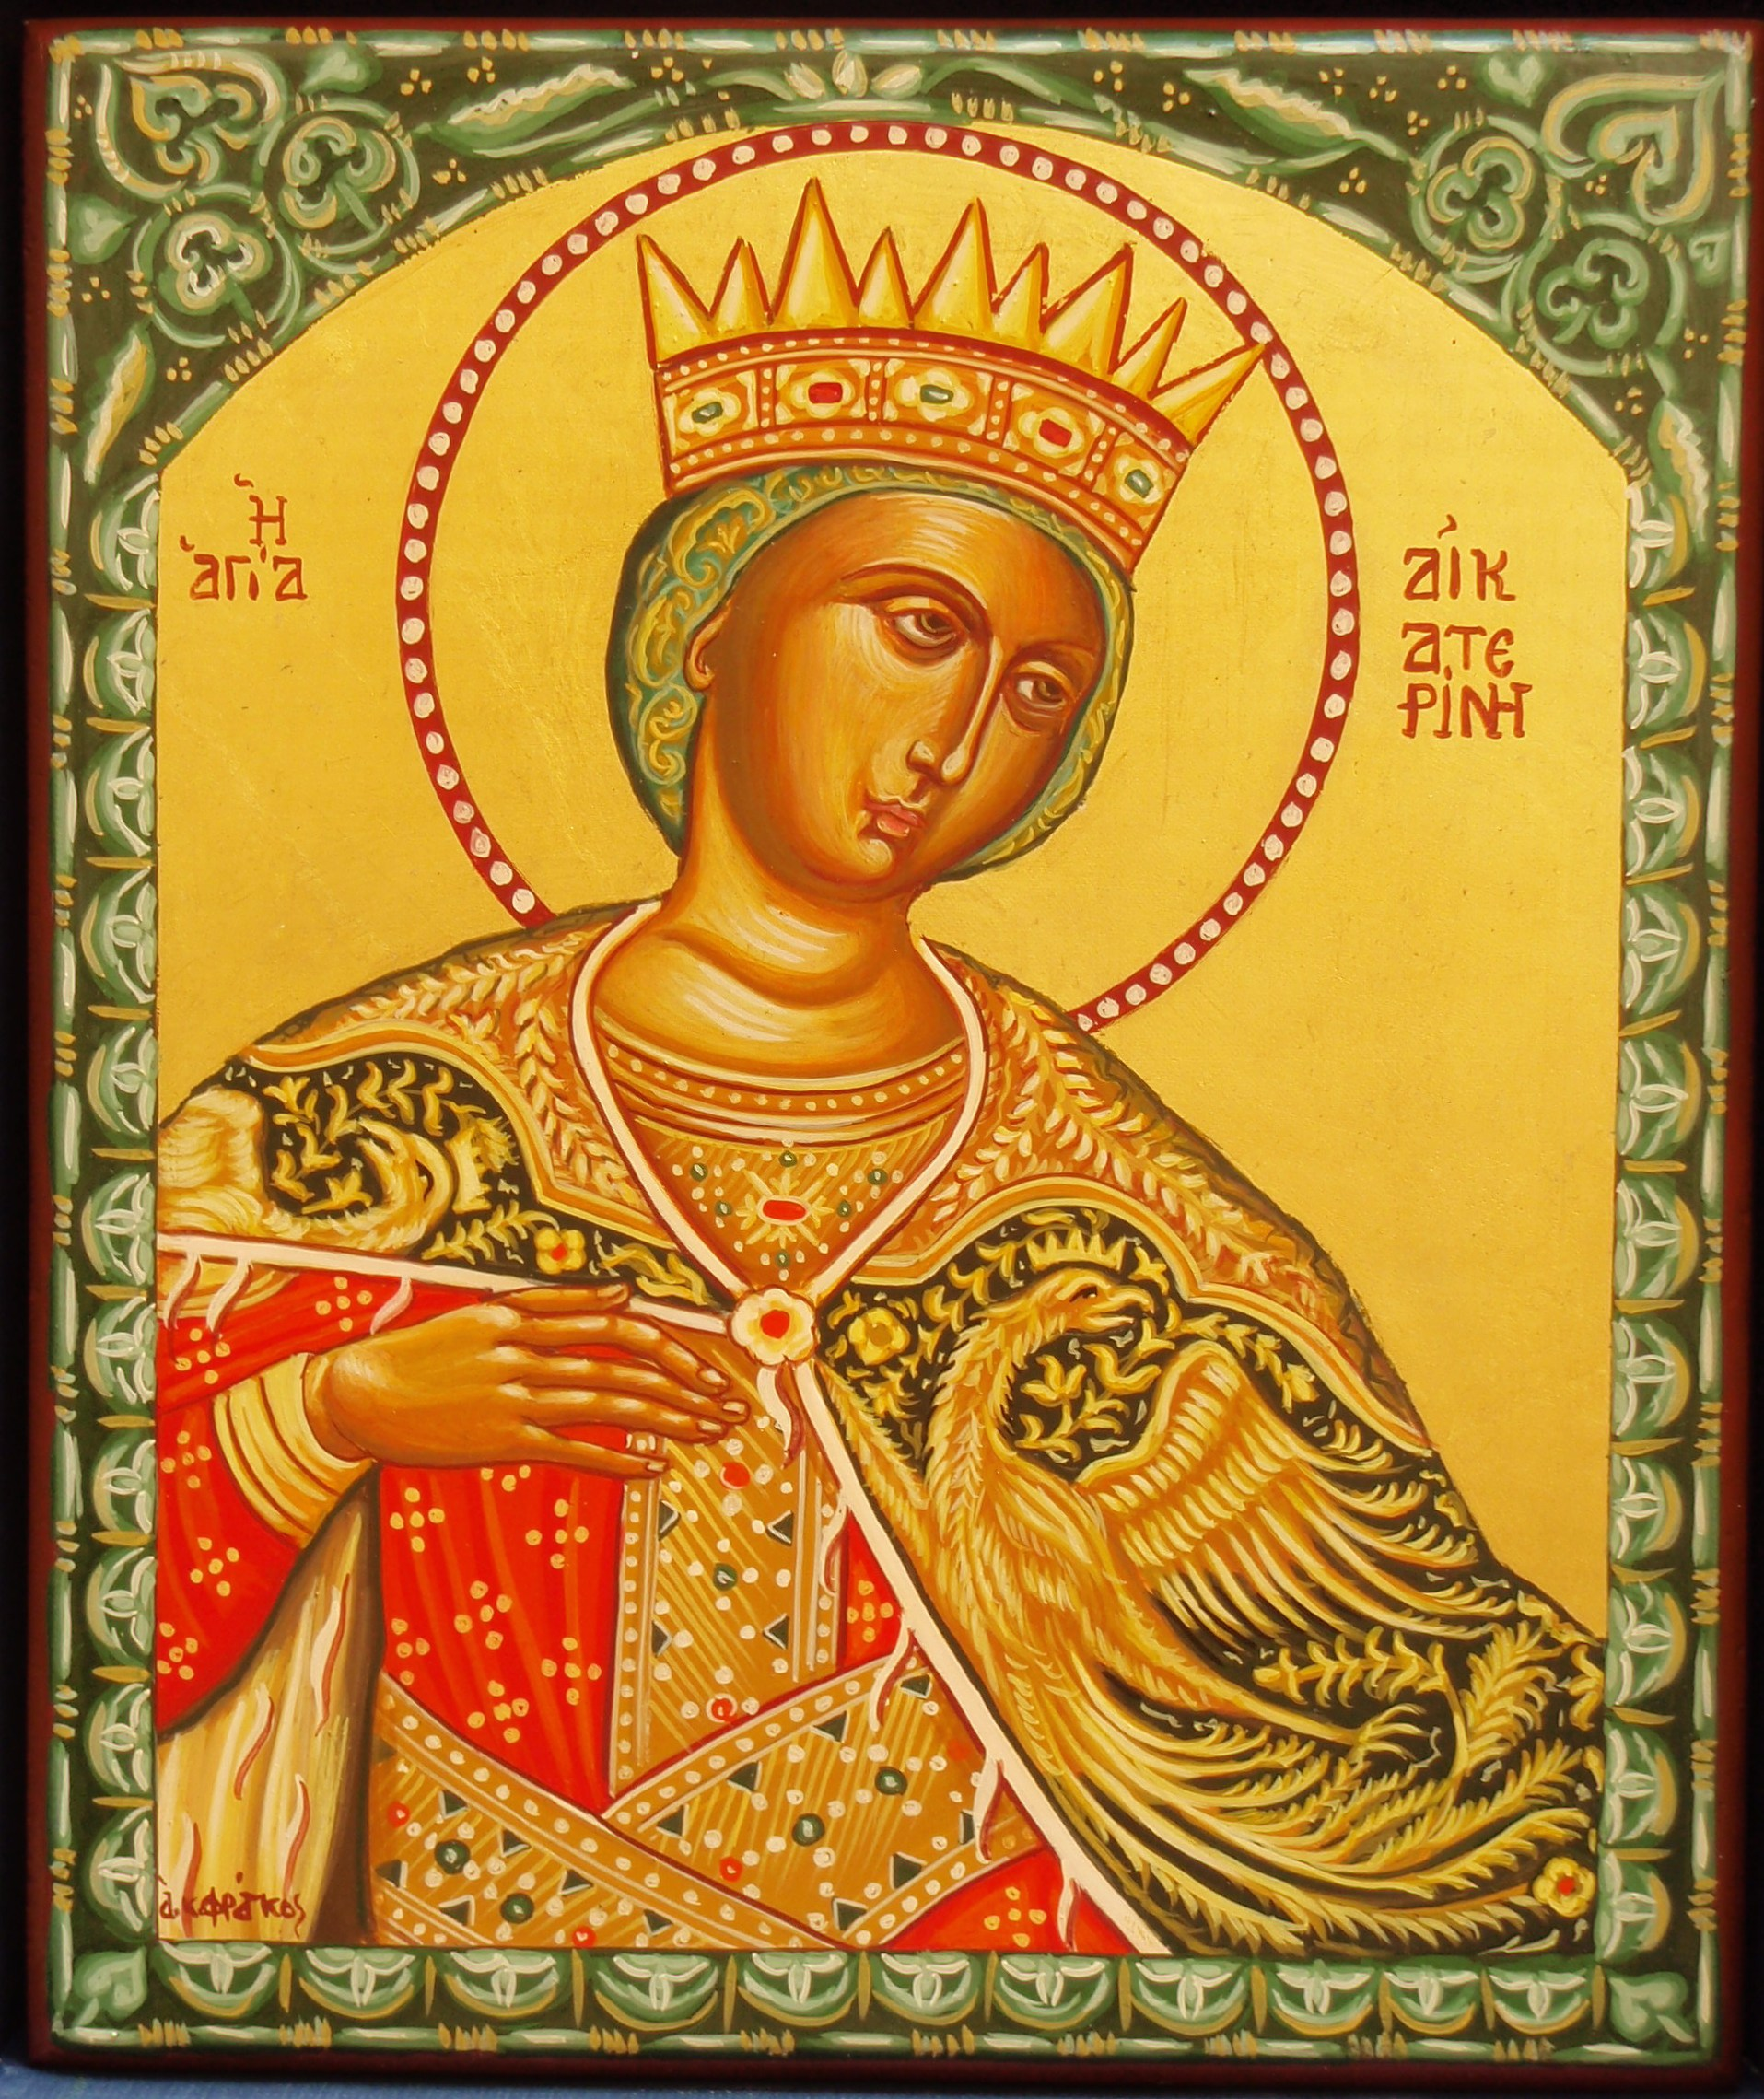
\includegraphics[width=0.5\textwidth]{Katherine1.jpg}}
\date{}
\author{}

\begin{document}
\maketitle
\instruction{This page intentionally left blank}
\cleardoublepage

\chapter*{The Sunday Reader's Service of Typica}
\readerline{Through the prayers of our holy fathers, Lord Jesus Christ our God,
  have mercy on us, and save us}
\lilypondfile{./Z-Responses/Obikhod/Amen.ly}
\readerline{\lhmTwelve}


\centeredsection{The First Antiphon}
\instruction{This may be replaced for certain feast days.}
\lilypondfile{./Liturgy/B-FirstAntiphon/BlessTheLord_Greek-Music.ly}
\readerline{\lhmThree}


\centeredsection{The Second Antiphon}
\instruction{This may be replaced for certain feast days.}
\lilypondfile{./Liturgy/C-SecondAntiphon/PraiseTheLord_Greek-Music.ly}
\readerline{\lhmThree}


\centeredsection{The Third Antiphon}
\instruction{This may be replaced for certain feast days.}
\lilypondfile{./Liturgy/D-ThirdAntiphon/Beatitudes_Moscow-Music.ly}

\centeredsection{The Entrance Hymn}
\readerline{ Let us attend!}
\lilypondfile{./Liturgy/E-LittleEntrance/Entrance_Russian-Music.ly}


\centeredsection{Apolytikion}
\instruction{This is modified on Great Feasts.}

\emph{The Sunday Apolytikion of the Resurrection.}

\readerline{\glory}

\emph{The appointed Apolytikion of the day.}

\readerline{\nowandever}


\centeredsection{The Tropar of Saint Katherine}
\lilypondfile{./Menaion/11-25-StKatherine/Katherine-Trop_Obikhod-Music.ly}
\readerline{\throughtheprayers}
\lilypondfile{./Z-Responses/Obikhod/Amen.ly}


\centeredsection{The Trisagion Hymn}
\lilypondfile{./Liturgy/I-ThriceHolyHymn/Trisagion_Arabic_a.ly}
\readerline{With Strength!}
\lilypondfile{./Liturgy/I-ThriceHolyHymn/Trisagion_Arabic_b.ly}


\centeredsection{The Prokeimenon}
\paragraph{Reader 1}{Let us attend!}

\instruction{The second reader should be standing in front of the royal doors facing the altar}
\paragraph{Reader 2} The Prokeimenon!

\instruction{The reader then intones the prokeimenon while facing the altar}


\centeredsection{The Epistle}
\paragraph{Reader 1} Wisdom!

\instruction{The second reader continues facing the altar}
\paragraph{Reader 2} The reading from the Epistle of the holy Apostle Paul to the
  \underline{\hspace{1in}}
  
  (or from the Acts of the Holy Apostles.)
  
  (or from the Holy Epistle of Saint \underline{\hspace{1cm}}.)

\paragraph{Reader 1} Let us attend.

\instruction{The Reader turns and faces the people, and then chants the appointed Epistle,
  or Epistles for the day.}

\instruction{Melody sung together while the Reader turns again to face the altar}
\lilypondfile{./Liturgy/J-EpistleGospel/Alleluarion-A_Alaska-Music.ly}

\instruction{The reader recites the first verse of the Alleluarion
             - Choir responds with harmonized verse}
\lilypondfile{./Liturgy/J-EpistleGospel/Alleluarion-B_Alaska-Music.ly}

\instruction{The reader recites the second verse of the Alleluarion and reverently returns to the congregation
             - Choir responds with wide harmonized verse}
\lilypondfile{./Liturgy/J-EpistleGospel/Alleluarion-C_Alaska-Music.ly}

\centeredsection{The Gospel}
\instruction{The reader appointed to read the gospel stands in front of the Royal Doors facing the people}
\readerline{Let us attend, the reading from the Holy Gospel according to Saint
  \underline{\hspace{1in}}.}
\lilypondfile{./Liturgy/J-EpistleGospel/GloryToThee_Kievan-Music.ly}

\readerline{\instruction{Gospel reading for the day}}
\lilypondfile{./Liturgy/J-EpistleGospel/GloryToThee_Kievan-Music.ly}

\begin{reader}
\item Lord, have mercy. \instruction{3x - (Said in place of the litany of the catechumens)}
\item Lord, have mercy. \instruction{3x - (Said in place of the first litany of the faithful)}
\item Lord, have mercy. \instruction{3x - (Said in place of the second litany of the faithful)}
\end{reader}


\centeredsection{Prayer to the Lord of Hosts}
\newcommand\metania{\emph{(metania)}}
Remember us, O Lord, when thou comest in thy kingdom.\metania

Remember us, O Master, when thou comest in thy kingdom.\metania

Remember us, O Holy One, when thou comest in thy kingdom.\metania

The heavenly choir singeth thy praises, saying: Holy, holy, holy, Lord of Sabaoth; heaven and earth are full of Thy glory.

Come unto him, and be enlightened, and your faces shall not be ashamed.

The heavenly choir singeth thy praises, saying: Holy, holy, holy, Lord of Sabaoth; heaven and earth are full of Thy glory.

\emph{\glory}

The choir of the holy angels and archangels, with all the powers of heaven, singeth thy praises, saying: Holy, holy, holy, Lord of Sabaoth; heaven and earth are full of Thy glory.

\emph{\nowandever}


\centeredsection{The Creed}
\input{Common/TheCreed.txt}


\centeredsection{Prayer of Forgiveness}
\readerline{Forgive, remit, pardon, O God, our sins,
  both voluntary and involuntary, in deed and in word, in knowledge or in ignorance,
  committed by night or by day, in mind and in thought.
  Forgive us them all, for thou art good and lovest mankind.
}


\centeredsection{The Lord’s Prayer}
\input{Common/LordsPrayer.txt}

\readerline{Through the prayers of our holy fathers, Lord Jesus Christ our God, have mercy on us.}
\lilypondfile{./Z-Responses/Obikhod/Amen.ly}


\centeredsection{Kontakia}
\instruction{This is modified on Great Feasts.}

\centeredsubsection{Kontakion of Saint Katherine}
\lilypondfile{./Menaion/11-25-StKatherine/Katherine-Kont_Obikhod-Music.ly}

\emph{The appointed Kontakion of the day.}

\readerline{\glory}

\emph{The Sunday Kontakion of the Resurrection.}

\readerline{\nowandever}

\centeredsubsection{Theotokion for Ordinary Sundays}
\instruction{This is often replaced with a Theotokion specific to the day.}

\lilypondfile{./Liturgy/H-Kontakion/OProtectionOfChristians_Greek-Music.ly}

\readerline{\lhmForty}

\lilypondfile{./Liturgy/Z-PostCommunionHymns/BlessedBeTheName_Plain-Music.ly}

\readerline{\gne}

\begin{maybetwocolumns}
\centeredsection{Psalm 33}
\input{./Psalms/Psalm033-unknowntrans.txt}

\centeredsection{Psalm 144}
\input{./Psalms/Psalm144-unknowntrans.txt}
\end{maybetwocolumns}

\readerline{\gne}


\centeredsection{The Theotokion}
\lilypondfile{./Liturgy/S-Megalynarion/ItIsTrulyMeet_Obikhod-Music.ly}


\centeredsection{}{The Dismissal}

\lilypondfile{./Z-Responses/Obikhod/GNE-Amen.ly}
\lilypondfile{./Z-Responses/Obikhod/LordHaveMercyX3-OLordBless.ly}
\readerline{\throughtheprayers}

\lilypondfile{./Z-Responses/Obikhod/Amen.ly}

\end{document}

